\section{计算张量网络的梯度}\label{chapter:gradients}
在一般情形下优化张量网络，是许多研究领域共同面临的重大挑战。针对矩阵的优化技术虽已发展良多，但把这些方法推广到张量网络仍然不易~\citep{liao2019differentiable}。其困难源于张量收缩的高昂计算代价，也源于高维情形缺少高效的优化算法。此外，只要张量网络的结构略微复杂，手工用链式法则求梯度便令人却步。本章介绍一种优雅而直观的方法：借助张量网络的图示记法来推导高阶导数。该方法表明，张量网络函数的导数往往继承初始张量网络的低秩结构。

下一节先针对以向量为输入的函数，给出梯度与雅可比矩阵（Jacobian）的经典概念，再把它们推广到以张量为输入、以张量为输出的函数。
\subsection{雅可比矩阵}
我们先回顾定义在 $\mathbb{R}^n$ 上的函数的梯度与雅可比矩阵这两个经典概念。

\begin{definition}
  设 $f:\RR^n\to\RR$ 与 $g:\RR^n\to\RR^p$。$f$ 的梯度与 $g$ 在 $\theta\in\mathbb{R}^n$ 处的雅可比矩阵定义为
    $$\nabla_\theta f = \left[\frac{\partial f(\theta)}
{\partial\theta_1},\frac{\partial f(\theta)}{\partial\theta_2},\dots,\frac{\partial f(\theta)} 
    {\partial\theta_n}\right]^\ts
        =
    \begin{tikzpicture}[baseline=\baseline]
    \tikzset{tensor/.style = {minimum size = 0.5cm,shape = circle,thick,draw=black,inner sep = 0pt}, edge/.style   = {thick,line width=.4mm}}
    \def\y{0}
     \def\x{0}
    \node[tensor,fill=blue!40!red!60!white] (a1) at (\x,\y){};
    \draw[edge](a1) -- (\x+0.75,\y)node [midway, above]{\edgelabel{$n$}};
    \end{tikzpicture} \in\mathbb{R}^n,$$
    以及
    $$\frac{\partial g(\theta)}{\partial\theta} = \left(\frac{\partial g(\theta)_i}{\partial\theta_j}\right)_{i=1,\cdots,p\atop j=1,\cdots, n}
    =
    \begin{tikzpicture}[baseline=\baseline]
    \tikzset{tensor/.style = {minimum size = 0.5cm,shape = circle,thick,draw=black,inner sep = 0pt}, edge/.style   = {thick,line width=.4mm}}
    \def\y{0}
     \def\x{0}
    \node[tensor,fill=blue!20!red!50!white] (A) at (\x,\y){};
    \draw[edge](A) -- (\x+0.75,\y)node [midway, above]{\scalebox{0.7}{\dimcolor{$n$}}};
    \draw[edge](A) -- (\x-0.75,\y)node [midway, above]{\scalebox{0.7}{\dimcolor{$p$}}};
    \end{tikzpicture}\in\mathbb{R}^{p\times n}.$$  
\end{definition}
雅可比矩阵的概念可以自然推广到以张量为输入、输出张量（阶数任意）的函数。

\begin{definition}
 设 $f:\RR^{n_1\times\dots\times n_N}\to\RR^{m_1\times\dots\times m_M}$，。$f$ 在 $\theta\in\RR^{n_1\times\dots\times n_N}$ 处的\emph{雅可比张量}是张量 $\frac{\partial f}{\partial\theta}\in\RR^{m_1\times\dots\times m_M\times n_1\times\dots\times n_N}$
 定义为
\begin{align*}
   \frac{\partial f(\theta)}{\partial\theta} 
   &= 
   \left(\frac{\partial f(\theta)_{i_1,\dots,i_M}}{\partial\theta_{j_1,\dots,j_N}}\right)_{i_1\in[m_1],\cdots,i_M\in[m_M]\atop j_1\in[n_1],\cdots,j_N
\in[n_N]}\\
&=
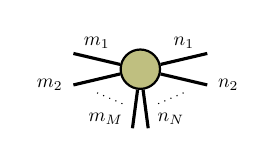
\begin{tikzpicture}[baseline=-0.5ex]
    \tikzset{tensor/.style = {minimum size = 0.5cm,shape = circle,thick,draw=black,inner sep = 0pt}, edge/.style = {thick,line width=.4mm},every loop/.style={}}
    \def\x{6}
    \node[tensor,fill=green!50!red!50!white] (T) at (\x,0) {};
    \draw[edge] (T) -- (\x-0.85,0.2)node [midway, above]{\scalebox{0.7}{\dimcolor{$m_1$}}};
    \draw[edge] (T) -- (\x-0.85,-0.2)node [left]{\scalebox{0.7}{\dimcolor{$m_2$}}};
    \draw[edge] (T) -- (\x-0.1,-0.75)node [near end, left]{\scalebox{0.7}{\dimcolor{$m_M$}}};
    \draw[dotted] (\x-0.55,-0.3) -- (\x-0.2,-0.45);
    \draw[edge] (T) -- (\x+0.85,0.2)node [midway, above]{\scalebox{0.7}{\dimcolor{$n_1$}}};
    \draw[edge] (T) -- (\x+0.85,-0.2)node [right]{\scalebox{0.7}{\dimcolor{$n_2$}}};
    \draw[edge] (T) -- (\x+0.1,-0.75)node [near end, right]{\scalebox{0.7}{\dimcolor{$n_N$}}};
    \draw[dotted] (\x+0.55,-0.3) -- (\x+0.2,-0.45);
    \end{tikzpicture}\in\RR^{m_1\times\cdots\times m_M\times n_1\times\cdots\times n_N}. 
\end{align*}
\end{definition}




下面的定理表明，张量网络关于某个核心张量的一阶导数，用张量网络本身就能轻松算出。

\begin{theorem}\label{thm:gradients}
    设 $\Tt$ 是由张量网络给出的张量，其中 $\Gt$ 是在该张量网络中\emph{只出现一次}的核心张量。那么，把 $\Gt$ 从 $\Tt$ 的张量网络中移除，所得即 $\frac{\partial \Tt}{\partial \Gt}$。 
\end{theorem}
下面的例子说明如何将定理~\ref{thm:gradients}用于张量网络。
\paragraph{示例}
设 
$\begin{tikzpicture}[baseline=\baseline]
    \tikzset{tensor/.style = {minimum size = 0.5cm,shape = circle,thick,draw=black,inner sep = 0pt}, edge/.style = {thick,line width=.4mm},every loop/.style={}}
    \def\x{0}
    \def\y{0}
     \node[tensor,fill=green!50!red!50!white] (B) at (\x+1,\y) {$\Xt$};
    \draw[edge] (B) -- (\x+0.25,0) node [midway,above] {\scalebox{0.7}{\dimcolor{$d_1$}}};
    \draw[edge] (B) -- (\x+1.85,\y) node [midway,above] {\scalebox{0.7}{\dimcolor{$d_3$}}};
    \draw[edge] (B) -- (\x+1,\y-0.85) node [midway,left] {\scalebox{0.7}{\dimcolor{$d_2$}}};
\end{tikzpicture}
=
\begin{tikzpicture}[baseline=\baseline]
    \tikzset{tensor/.style = {minimum size = 0.5cm,shape = circle,thick,draw=black,inner sep = 0pt}, edge/.style = {thick,line width=.4mm},every loop/.style={}}
    \def\x{0}
    \def\y{0}
    \node[tensor,fill=red!30!white] (A) at (\x+2,\y) {$\Gt_1$};
    \node[tensor,fill=red!50!white] (B) at (\x+3.2,\y) {$\Gt_2$};
    \node[tensor,fill=blue!30!white] (C) at (\x+2.6,\y-0.7) {$\Gt_3$};
    \node[tensor,fill=blue!50!white] (D) at (\x+4.3,\y) {$\Gt_4$};
    \draw[edge] (A) -- (B) node [midway,above] {\scalebox{0.7}{\dimcolor{$R_1$}}};
    \draw[edge] (A) -- (C);
    \node[draw=none] () at (\x+2,\y-0.5) {\scalebox{0.7}{\dimcolor{$R_2$}}};
    \draw[edge] (B) -- (C);
    \node[draw=none] () at (\x+3.2,\y-0.5) {\scalebox{0.7}{\dimcolor{$R_3$}}};
    \draw[edge] (B) -- (D) node [midway,above] {\scalebox{0.7}{\dimcolor{$R_4$}}};
    \draw[edge] (A) -- (\x+2,\y+0.7) node [midway,left] {\scalebox{0.7}{\dimcolor{$d_1$}}};
    \draw[edge] (D) -- (\x+4.3,\y+0.7) node [midway,right] {\scalebox{0.7}{\dimcolor{$d_3$}}};
    \draw[edge] (C) -- (\x+2.6,\y-1.5) node [midway,left] {\scalebox{0.7}{\dimcolor{$d_2$}}};
\end{tikzpicture}
$ 为张量网络。注意，可以把 $\Xt$ 看作其张量网络表示中任一核心张量的函数，于是自然会问：$\Xt$ 关于例如 $\Gt_2$ 或 $\Gt_4$ 的雅可比矩阵是什么。
上述定理给出了计算这些导数的简便途径：
\begin{itemize}
\item 根据定理~\ref{thm:gradients}，要求 $\Xt$ 关于 $\Gt_2$ 的梯度，需从张量网络中移除核心张量 $\Gt_2$，即
$$
\frac{\partial}{\partial\Gt_2}\left(\begin{tikzpicture}[baseline=\baseline]
    \tikzset{tensor/.style = {minimum size = 0.5cm,shape = circle,thick,draw=black,inner sep = 0pt}, edge/.style = {thick,line width=.4mm},every loop/.style={}}
    \def\y{0}
    \def\x{0}
    \node[tensor,fill=red!30!white] (A) at (\x+2,\y) {$\Gt_1$};
    \node[tensor,fill=red!50!white] (B) at (\x+3.2,\y) {$\Gt_2$};
    \node[tensor,fill=blue!30!white] (C) at (\x+2.6,\y-0.7) {$\Gt_3$};
    \node[tensor,fill=blue!50!white] (D) at (\x+4.3,\y) {$\Gt_4$};
    \draw[edge] (A) -- (B) node [midway,above] {\scalebox{0.7}{\dimcolor{$R_1$}}};
    \draw[edge] (A) -- (C);
    \node[draw=none] () at (\x+2,\y-0.5) {\scalebox{0.7}{\dimcolor{$R_2$}}};
    \draw[edge] (B) -- (C);
    \node[draw=none] () at (\x+3.2,\y-0.5) {\scalebox{0.7}{\dimcolor{$R_3$}}};
    \draw[edge] (B) -- (D) node [midway,above] {\scalebox{0.7}{\dimcolor{$R_4$}}};
    \draw[edge] (A) -- (\x+2,\y+0.7) node [midway,left] {\scalebox{0.7}{\dimcolor{$d_1$}}};
    \draw[edge] (D) -- (\x+4.3,\y+0.7) node [midway,right] {\scalebox{0.7}{\dimcolor{$d_3$}}};
    \draw[edge] (C) -- (\x+2.6,\y-1.5) node [midway,left] {\scalebox{0.7}{\dimcolor{$d_2$}}};
    \end{tikzpicture}\right)
=
    \begin{tikzpicture}[baseline=\baseline]
    \tikzset{tensor/.style = {minimum size = 0.5cm,shape = circle,thick,draw=black,inner sep = 0pt}, edge/.style = {thick,line width=.4mm},every loop/.style={}}
    \def\y{-0.5}
    \def\x{0}
    \node[tensor,fill=red!30!white] (A) at (\x,\y+1) {$\Gt_1$};
    \node[tensor,fill=blue!30!white] (C) at (\x+0.6,\y+0.2) {$\Gt_3$};
    \node[tensor,fill=blue!50!white] (D) at (\x+2,\y+0.5) {$\Gt_4$};
    \draw[edge] (A) -- (C);
    \draw[edge] (A) -- (\x,\y+1.7) node [midway,left] {\scalebox{0.7}{\dimcolor{$d_1$}}};
    \draw[edge] (A) -- (\x+0.7,\y+1) node [midway,above] 
{\scalebox{0.7}{\dimcolor{$R_1$}}};
    \draw[edge] (D) -- (\x+3,\y+0.5) node [midway,above] {\scalebox{0.7}{\dimcolor{$R_4$}}};
    \draw[edge] (C) -- (\x+0.6,\y-0.7) node [midway,left] {\scalebox{0.7}{\dimcolor{$d_2$}}};
    \draw[edge] (C) -- (\x+1.3,\y+0.2) node [midway,above] {\scalebox{0.7}{\dimcolor{$R_3$}}};
    \draw[edge] (D) -- (\x+2,\y+1.3) node [midway,left] {\scalebox{0.7}{\dimcolor{$d_3$}}};
    \node[draw=none] () at (\x,\y+0.4) {\scalebox{0.7}{\dimcolor{$R_2$}}};
\end{tikzpicture}.
$$ 
要理解这一做法为何成立，可把 $\Xt$ 的张量分解看作矩阵-向量乘积：
$$
\Mb\vb 
=
\begin{tikzpicture}[baseline=\baseline]
    \tikzset{tensor/.style = {minimum size = 0.5cm,shape = circle,thick,draw=black,inner sep = 0pt}, edge/.style = {thick,line width=.4mm},every loop/.style={}}
    \def\y{1}
    \def\x{0}
     \node[tensor,fill=red!30!white](G_1) at (\x,\y) {$\Gt_1$};
    \node[tensor,fill=blue!30!white] (G_3) at (\x,\y-1) {$\Gt_3$};
     \node[tensor,fill=red!50!white](G_2) at (\x+2,\y-1) {$\Gt_2$};
    \node[tensor,fill=blue!50!white] (G_4) at (\x,\y-2) {$\Gt_4$};
    \node[tensor,fill=red!50!white] (G_2) at (\x+2,\y-1) {$\Gt_2$};
    \draw[edge](G_1) -- (\x-1,\y) -- (\x-1,\y-0.85) -- (\x-1.75,\y-0.85);
    \draw[edge](G_3)-- (\x-1.75,\y-1)node [left] {\scalebox{0.7}{\dimcolor{$d_1d_2d_3$}}};
    \draw[edge](G_2)--(G_1)node [midway,above] {\scalebox{0.7}{\dimcolor{$R_1$}}};
    \draw[edge](G_2)--(G_3)node [midway,above] {\scalebox{0.7}{\dimcolor{$R_3$}}};
    \draw[edge](G_1)--(G_3)node [midway,left] {\scalebox{0.7}{\dimcolor{$R_2$}}};
    \draw[edge](G_2)--(G_4)node [midway,above] {\scalebox{0.7}{\dimcolor{$R_4$}}};
    \draw[edge] (G_4) -- (\x-1,\y-2) -- (\x-1,\y-1.15) -- (\x-1.75,\y-1.15);
    \draw[dotted] (\x+0.45,\y+0.65) -- (\x+0.45,\y-2.35);
\end{tikzpicture},
$$
其中 $\vb = \vectorize(\Gt_2) $，而 $\Mb$ 是把张量网络余下部分矩阵化后得到的矩阵。 
利用线性映射的雅可比矩阵这一经典恒等式，便得到期望的结果：
$$\frac{\partial\Mb\vb}{\partial\vb} = \Mb = 
\begin{tikzpicture}[baseline=\baseline]
    \tikzset{tensor/.style = {minimum size = 0.5cm,shape = circle,thick,draw=black,inner sep = 0pt}, edge/.style = {thick,line width=.4mm},every loop/.style={}}
    \def\y{1}
    \def\x{0}
     \node[tensor,fill=red!30!white](G_1) at (\x,\y) {$\Gt_1$};
    \node[tensor,fill=blue!30!white] (G_3) at (\x,\y-1) {$\Gt_3$};
    \node[tensor,fill=blue!50!white] (G_4) at (\x,\y-2) {$\Gt_4$};
    \draw[edge](G_1) -- (\x-0.85,\y) -- (\x-0.85,\y-0.9) -- (\x-1.5,\y-0.9);
    \draw[edge](G_3)-- (\x-1.5,\y-1)node [left] {\scalebox{0.7}{\dimcolor{$d_1d_2d_3$}}};
    \draw[edge](G_1)-- (\x+0.85,\y) -- (\x+0.85,\y-0.9) -- (\x+1.5,\y-0.9);
    \draw[edge](G_3) -- (\x+1.5,\y-1) node [right] {\scalebox{0.7}{\dimcolor{$R_1R_3R_4$}}};
    \draw[edge](G_1)--(G_3)node [midway,left] {\scalebox{0.7}{\dimcolor{$R_2$}}};
    \draw[edge] (G_4) -- (\x+0.85,\y-2) -- (\x+0.85,\y-1.1) -- (\x+1.5,\y-1.1);
    \draw[edge] (G_4) -- (\x-0.85,\y-2) -- (\x-0.85,\y-1.1) -- (\x-1.5,\y-1.1);
\end{tikzpicture}\in\RR^{d_1d_2d_3\times R_1R_3R_4}.
$$
\item 根据定理~\ref{thm:gradients}，要求 $\Xt$ 关于 $\Gt_4$ 的梯度，需从相应的张量网络中移除核心张量 $\Gt_4$。即 
$$
    \frac{\partial}{\partial\Gt_4}\left(\begin{tikzpicture}[baseline=\baseline]
    \tikzset{tensor/.style = {minimum size = 0.5cm,shape = circle,thick,draw=black,inner sep = 0pt}, edge/.style = {thick,line width=.4mm},every loop/.style={}}
    \def\x{0}
    \def\y{0}
    \node[tensor,fill=red!30!white] (A) at (\x+2,\y) {$\Gt_1$};
    \node[tensor,fill=red!50!white] (B) at (\x+3.2,\y) {$\Gt_2$};
    \node[tensor,fill=blue!30!white] (C) at (\x+2.6,\y-0.7) {$\Gt_3$};
    \node[tensor,fill=blue!50!white] (D) at (\x+4.3,\y) {$\Gt_4$};
    \draw[edge] (A) -- (B) node [midway,above] {\scalebox{0.7}{\dimcolor{$R_1$}}};
    \draw[edge] (A) -- (C);
    \node[draw=none] () at (\x+2,\y-0.5) {\scalebox{0.7}{\dimcolor{$R_2$}}};
    \draw[edge] (B) -- (C);
    \node[draw=none] () at (\x+3.2,\y-0.5) {\scalebox{0.7}{\dimcolor{$R_3$}}};
    \draw[edge] (B) -- (D) node [midway,above] {\scalebox{0.7}{\dimcolor{$R_4$}}};
    \draw[edge] (A) -- (\x+2,\y+0.7) node [midway,left] {\scalebox{0.7}{\dimcolor{$d_1$}}};
    \draw[edge] (D) -- (\x+4.3,\y+0.7) node [midway,right] {\scalebox{0.7}{\dimcolor{$d_3$}}};
    \draw[edge] (C) -- (\x+2.6,\y-1.5) node [midway,left] {\scalebox{0.7}{\dimcolor{$d_2$}}};
    \end{tikzpicture}\right)
=
    \begin{tikzpicture}[baseline=\baseline]
    \tikzset{tensor/.style = {minimum size = 0.5cm,shape = circle,thick,draw=black,inner sep = 0pt}, edge/.style = {thick,line width=.4mm},every loop/.style={}}
    \def\y{-0.5}
    \def\x{0}
    \node[tensor,fill=red!30!white] (A) at (\x+2,\y+1) {$\Gt_1$};
    \node[tensor,fill=red!50!white] (B) at (\x+3.2,\y+1) {$\Gt_2$};
    \node[tensor,fill=blue!30!white] (C) at (\x+2.6,\y) {$\Gt_3$};
    \draw[edge] (A) -- (B) node [midway,above] {\scalebox{0.7}{\dimcolor{$R_1$}}};
    \draw[edge] (A) -- (C);
    \node[draw=none] () at (\x+2,\y+0.5) {\scalebox{0.7}{\dimcolor{$R_2$}}};
    \draw[edge] (B) -- (C);
    \node[draw=none] () at (\x+3.2,\y+0.5) {\scalebox{0.7}{\dimcolor{$R_3$}}};
    \draw[edge] (B) -- (\x+4,\y+1) node [midway,above] {\scalebox{0.7}{\dimcolor{$R_4$}}};
    \draw[edge] (A) -- (\x+2,\y+1.7) node [midway,left] {\scalebox{0.7}{\dimcolor{$d_1$}}};
    \draw[edge] (C) -- (\x+2.6,\y-0.7) node [midway,left] {\scalebox{0.7}{\dimcolor{$d_2$}}};
    \draw[edge] (\x+4.5,\y+1) -- (\x+4.5,\y+1.65) node [midway,right] {\scalebox{0.7}{\dimcolor{$d_3$}}};
    \end{tikzpicture}.
$$
注意 $\Gt_4$ 的悬空腿（dangling leg）仍留在雅可比张量中！为理解这一点，可再次把 $\Xt$ 的张量分解看作矩阵-向量乘积 $\Mb\vb$，使得 
$$
\Mb\vb = \begin{tikzpicture}[baseline=\baseline]
    \tikzset{tensor/.style = {minimum size = 0.5cm,shape = circle,thick,draw=black,inner sep = 0pt}, edge/.style = {thick,line width=.4mm},every loop/.style={}}
    \def\y{0.7}
    \def\x{0}
     \node[tensor,fill=red!30!white](G_1) at (\x,\y) {$\Gt_1$};
     \node[tensor,fill=red!50!white](G_2) at (\x+1,\y) {$\Gt_2$};
    \node[tensor,fill=blue!30!white] (G_3) at (\x+0.5,\y-1) {$\Gt_3$};
    \node[tensor,fill=blue!50!white] (G_4) at (\x+2.25,\y-1.5) {$\Gt_4$};
    \draw[edge](G_2)--(G_3);
    \draw[edge](G_1)--(G_2)node [midway,above] {\scalebox{0.7}{\dimcolor{$R_1$}}};
    \draw[edge](G_1)--(G_3);
    \draw[edge](G_2)--(G_4)node [midway,above=0.05cm] {\scalebox{0.7}{\dimcolor{$R_4$}}};
    \draw[edge](G_1) -- (\x,\y-1.35) -- (\x+0.35,\y-1.35) -- (\x+0.35,\y-2);
    \draw[edge](G_3)--(\x+0.5,\y-2)node [below] {\scalebox{0.7}{\dimcolor{$d_1d_2d_3$}}};
    \draw[edge](G_4) -- (\x+0.75,\y-1.5) -- (\x+0.75,\y-2);
    \draw[dotted] (\x+2.25,\y-0.75) -- (\x+1,\y-2);
\end{tikzpicture},
$$
此时 $\vb  =\vectorize(\Gt_4)$。
对该张量网络关于 $\vb = \vectorize(\Gb_4)$ 求导，便得到期望的结果：  $$\frac{\partial\Mb\vb}{\partial\vb} = \Mb
=
\begin{tikzpicture}[baseline=\baseline]
\tikzset{tensor/.style = {minimum size = 0.5cm,shape = circle,thick,draw=black,inner sep = 0pt}, edge/.style = {thick,line width=.4mm},every loop/.style={}}
    \def\y{1}
    \def\x{0}
     \node[tensor,fill=red!30!white](G_1) at (\x,\y) {$\Gt_1$};
     \node[tensor,fill=red!50!white](G_2) at (\x+1,\y) {$\Gt_2$};
    \node[tensor,fill=blue!30!white] (G_3) at (\x+0.5,\y-1) {$\Gt_3$};
    \draw[edge](G_2)--(G_3);
    \draw[edge](G_1)--(G_2)node [midway,above] {\scalebox{0.7}{\dimcolor{$R_1$}}};
    \draw[edge](G_1)--(G_3);
    \draw[edge](G_1) -- (\x,\y-1.35) -- (\x+0.35,\y-1.35) -- (\x+0.35,\y-2);
    \draw[edge](G_3)--(\x+0.5,\y-2)node [below] {\scalebox{0.7}{\dimcolor{$d_1d_2d_3$}}};
     \draw[edge](G_2) -- (\x+1.85,\y)node [midway, above] {\scalebox{0.7}{\dimcolor{$R_4$}}};
    \draw[edge](\x+1.85,\y-1.5) -- (\x+0.75,\y-1.5) -- (\x+0.75,\y-2);
\end{tikzpicture}\in\RR^{d_1d_2d_3\times R_4}.$$
注意，对某个张量求导只是从网络中移除相应的节点，而与它相连的边（腿）保持原样。
\end{itemize}
下面说明如何用定理~\ref{thm:gradients}不费力气地推出经典的导数与梯度计算式。 
\paragraph{用张量网络重新推导经典恒等式}
\begin{enumerate}
\item 
    $\frac{\partial\langle\ub,\vb\rangle}{\partial \ub}
=
    \frac{\partial\left(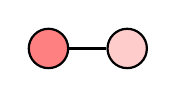
\begin{tikzpicture}[baseline=-0.1ex]
    \tikzset{tensor/.style = {minimum size = 0.5cm,shape = circle,thick,draw=black,inner sep = 0pt}, edge/.style = {thick,line width=.4mm},every loop/.style={}}
    \def\x{0}
    \def\y{0}
    \node[tensor,fill=red!50!white] (u) at (\x+1,\y) {$\ub$};
    \node[tensor,fill=red!20!white] (v) at (\x+2,\y) {$\vb$};
    \draw[edge] (u) -- (v);
    \end{tikzpicture}\right)}{\partial\left(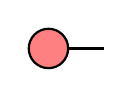
\begin{tikzpicture}[baseline=-0.1ex]
    \tikzset{tensor/.style = {minimum size = 0.5cm,shape = circle,thick,draw=black,inner sep = 0pt}, edge/.style = {thick,line width=.4mm},every loop/.style={}}
    \def\x{0}
    \def\y{0}
    \node[tensor,fill=red!50!white] (u) at (\x+1,\y) {$\ub$};
    \draw[edge] (u) -- (\x+1.7,\y);
    \end{tikzpicture}\right)}
=
    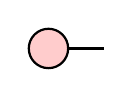
\begin{tikzpicture}[baseline=-0.1ex]
    \tikzset{tensor/.style = {minimum size = 0.5cm,shape = circle,thick,draw=black,inner sep = 0pt}, edge/.style = {thick,line width=.4mm},every loop/.style={}}
    \def\x{6}
    \def\y{0}
    \node[tensor,fill=red!20!white] (v) at (\x+2,\y) {$\vb$};
    \draw[edge] (v) -- (\x+2.7,\y);
    \end{tikzpicture}
    =
    \vb
    $
\item
    $\frac{\partial\Ab\xb}{\partial\xb}
=
    \frac{\partial\left(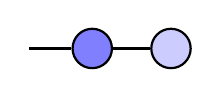
\begin{tikzpicture}[baseline=-0.1ex]
    \tikzset{tensor/.style = {minimum size = 0.5cm,shape = circle,thick,draw=black,inner sep = 0pt}, edge/.style = {thick,line width=.4mm},every loop/.style={}}
    \def\x{6}
    \def\y{0}
    \node[tensor,fill=blue!50!white] (A) at (\x+1,\y) {$\Ab$};
    \node[tensor,fill=blue!20!white] (x) at (\x+2,\y) {$\xb$};
    \draw[edge] (A) -- (x);
    \draw[edge] (A) -- (\x+0.2,\y);
    \end{tikzpicture}\right)}{\partial\left(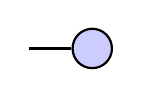
\begin{tikzpicture}[baseline=-0.1ex]
    \tikzset{tensor/.style = {minimum size = 0.5cm,shape = circle,thick,draw=black,inner sep = 0pt}, edge/.style = {thick,line width=.4mm},every loop/.style={}}
    \def\x{6}
    \def\y{0}
    \node[tensor,fill=blue!20!white] (x) at (\x+1,\y) {$\xb$};
    \draw[edge] (x) -- (\x+0.2,\y);
    \end{tikzpicture}\right)}
=
    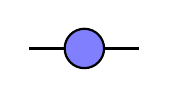
\begin{tikzpicture}[baseline=-0.1ex]
    \tikzset{tensor/.style = {minimum size = 0.5cm,shape = circle,thick,draw=black,inner sep = 0pt}, edge/.style = {thick,line width=.4mm},every loop/.style={}}
    \def\x{6}
    \def\y{0}
    \node[tensor,fill=blue!50!white] (A) at (\x+1,\y) {$\Ab$};
    \draw[edge] (A) -- (\x+0.3,\y);
    \draw[edge] (A) -- (\x+1.7,\y);
    \end{tikzpicture}
=
    \Ab
    $
    
\item 
    $\frac{\partial \xb^\ts\Ab\xb}{\partial\Ab}
=
    \frac{\partial\left(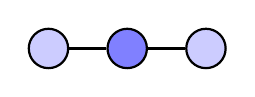
\begin{tikzpicture}[baseline=-0.1ex]
    \tikzset{tensor/.style = {minimum size = 0.5cm,shape = circle,thick,draw=black,inner sep = 0pt}, edge/.style = {thick,line width=.4mm},every loop/.style={}}
    \def\x{6}
    \def\y{0}
    \node[tensor,fill=blue!50!white] (A) at (\x+1,\y) {$\Ab$};
    \node[tensor,fill=blue!20!white] (x) at (\x+2,\y) {$\xb$};
    \node[tensor,fill=blue!20!white] (xt) at (\x,\y) {$\xb$};
    \draw[edge] (A) -- (x);
    \draw[edge] (A) -- (xt);
    \end{tikzpicture}\right)}{\partial\left(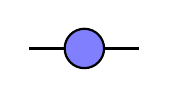
\begin{tikzpicture}[baseline=-0.1ex]
    \tikzset{tensor/.style = {minimum size = 0.5cm,shape = circle,thick,draw=black,inner sep = 0pt}, edge/.style = {thick,line width=.4mm},every loop/.style={}}
    \def\x{6}
    \def\y{0}
    \node[tensor,fill=blue!50!white] (A) at (\x+1,\y) {$\Ab$};
    \draw[edge] (A) -- (\x+1.7,\y);
    \draw[edge] (A) -- (\x+0.3,\y);
    \end{tikzpicture}\right)}
=
    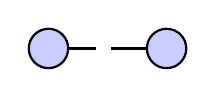
\begin{tikzpicture}[baseline=-0.1ex]
    \tikzset{tensor/.style = {minimum size = 0.5cm,shape = circle,thick,draw=black,inner sep = 0pt}, edge/.style = {thick,line width=.4mm},every loop/.style={}}
    \def\x{6}
    \def\y{0}
    \node[tensor,fill=blue!20!white] (x) at (\x+1,\y) {$\xb$};
    \node[tensor,fill=blue!20!white] (xt) at (\x-0.5,\y) {$\xb$};
    \draw[edge] (x) -- (\x+0.3,\y);
    \draw[edge] (xt) -- (\x+0.1,\y);
    \end{tikzpicture}
=
    \xb\outprod\xb
$
\item 
    $\frac{\partial\tr(\Ab)}{\partial\Ab}
    =
    \frac{\partial\left(
\begin{tikzpicture}[baseline=-0.1ex]
    \tikzset{tensor/.style = {minimum size = 0.5cm,shape = circle,thick,draw=black,inner sep = 0pt}, edge/.style = {thick,line width=.4mm},every loop/.style={}}
    \def\x{6}
    \def\y{0}
    \node[tensor,fill=blue!50!white] (A) at (\x+1,\y) {$\Ab$};
    \draw[edge] (A) to [out=20,in=160, distance=1cm] (A);
    \end{tikzpicture}\right)}
    {\partial\left(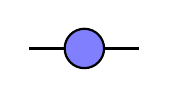
\begin{tikzpicture}[baseline=-0.1ex]
    \tikzset{tensor/.style = {minimum size = 0.5cm,shape = circle,thick,draw=black,inner sep = 0pt}, edge/.style = {thick,line width=.4mm},every loop/.style={}}
    \def\x{6}
    \def\y{0}
    \node[tensor,fill=blue!50!white] (A) at (\x+1,\y) {$\Ab$};
    \draw[edge] (A) -- (\x+1.7,\y);
    \draw[edge] (A) -- (\x+0.3,\y);
    \end{tikzpicture}\right)}
=

\begin{tikzpicture}[baseline=-0.1ex]
    \tikzset{tensor/.style = {minimum size = 0.5cm,shape = circle,thick,draw=black,inner sep = 0pt}, edge/.style = {thick,line width=.4mm},every loop/.style={}}
    \def\x{6}
    \def\y{0}
    \node[draw=none] (A) at (\x+1,\y) {};
    \draw[edge] (A) to [out=20,in=160, distance=1cm] (A);
    \end{tikzpicture}
=
    \Ib
    $
    \item
    $\frac{\partial\Ab\xb}{\partial\Ab}
=
    \frac{\partial\left(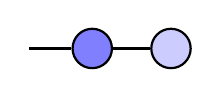
\begin{tikzpicture}[baseline=-0.1ex]
    \tikzset{tensor/.style = {minimum size = 0.5cm,shape = circle,thick,draw=black,inner sep = 0pt}, edge/.style = {thick,line width=.4mm},every loop/.style={}}
    \def\x{6}
    \def\y{0}
    \node[tensor,fill=blue!50!white] (A) at (\x+1,\y) {$\Ab$};
    \node[tensor,fill=blue!20!white] (x) at (\x+2,\y) {$\xb$};
    \draw[edge] (A) -- (x);
    \draw[edge] (A) -- (\x+0.2,\y);
    \end{tikzpicture}\right)}{\partial\left(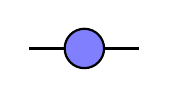
\begin{tikzpicture}[baseline=-0.1ex]
    \tikzset{tensor/.style = {minimum size = 0.5cm,shape = circle,thick,draw=black,inner sep = 0pt}, edge/.style = {thick,line width=.4mm},every loop/.style={}}
    \def\x{6}
    \def\y{0}
    \node[tensor,fill=blue!50!white] (A) at (\x+1,\y) {$\Ab$};
    \draw[edge] (A) -- (\x+0.3,\y);
    \draw[edge] (A) -- (\x+1.7,\y);
    \end{tikzpicture}\right)}
=
    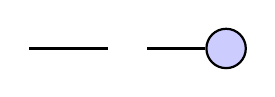
\begin{tikzpicture}[baseline=-0.1ex]
    \tikzset{tensor/.style = {minimum size = 0.5cm,shape = circle,thick,draw=black,inner sep = 0pt}, edge/.style = {thick,line width=.4mm},every loop/.style={}}
    \def\x{6}
    \def\y{0}
    \draw[edge] (\x+2,\y) -- (\x+3,\y);
    \node[tensor,fill=blue!20!white] (x) at (\x+4.5,\y) {$\xb$};
    \draw[edge] (x) -- (\x+3.5,\y);
    \node[draw=none] at (\x+3.25,\y){$\outprod$};
    \end{tikzpicture}
=
    \Ib\outprod\xb
$,
\end{enumerate}
其中最后一个恒等式的结果是三阶张量。
定理~\ref{thm:gradients}适用于被求导的张量在网络中只出现一次的情形。下面的定理说明如何处理同一张量出现多次的情形。
\begin{theorem}\label{thm:multiple-tensors-gradients}
    设 $\Tt$ 为张量网络，$\Gt$ 是其中的核心张量。若 $\Gt$ 在 $\Tt$ 的张量网络中出现 $k$ 次，则把 $\Tt$ 的张量网络的 $k$ 份拷贝相加，每份拷贝中移除 $\Gt$ 的一次不同出现，所得即 $\frac{\partial\Tt}{\partial\Gt}$。
\end{theorem}
下面的例子说明如何应用定理~\ref{thm:multiple-tensors-gradients}。
\paragraph{示例}
\begin{itemize}
    \item 设 $\xb\in\RR^{d}$，$\Ab\in\RR^{d\times d}$
    \begin{align*}
    \frac{\partial \xb^\ts\Ab\xb}{\partial\xb}
=
    \frac{\partial\left(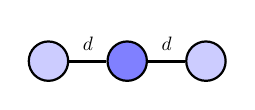
\begin{tikzpicture}[baseline=-0.1ex]
    \tikzset{tensor/.style = {minimum size = 0.5cm,shape = circle,thick,draw=black,inner sep = 0pt}, edge/.style = {thick,line width=.4mm},every loop/.style={}}
    \def\x{6}
    \def\y{0}
    \node[tensor,fill=blue!50!white] (A) at (\x+1,\y) {$\Ab$};
    \node[tensor,fill=blue!20!white] (x) at (\x+2,\y) {$\xb$};
    \node[tensor,fill=blue!20!white] (xprime) at 
    (\x,\y){$\xb$};
    \draw[edge] (A) -- (x)node [midway, above] {\scalebox{0.7}{\dimcolor{$d$}}};
    \draw[edge] (A) -- (xprime)node [midway, above] {\scalebox{0.7}{\dimcolor{$d$}}};
    \end{tikzpicture}\right)}{\partial\left(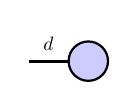
\begin{tikzpicture}[baseline=-0.1ex]
    \tikzset{tensor/.style = {minimum size = 0.5cm,shape = circle,thick,draw=black,inner sep = 0pt}, edge/.style = {thick,line width=.4mm},every loop/.style={}}
    \def\x{6}
    \def\y{0}
    \node[tensor,fill=blue!20!white] (x) at (\x,\y) {$\xb$};
    \draw[edge] (x) -- (\x-0.75,\y)node [midway, above] {\scalebox{0.7}{\dimcolor{$d$}}};
    \end{tikzpicture}\right)}
&=
    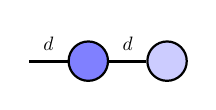
\begin{tikzpicture}[baseline=-0.1ex]
    \tikzset{tensor/.style = {minimum size = 0.5cm,shape = circle,thick,draw=black,inner sep = 0pt}, edge/.style = {thick,line width=.4mm},every loop/.style={}}
    \def\x{6}
    \def\y{0}
    \node[tensor,fill=blue!50!white] (A) at (\x+1,\y) {$\Ab$};
    \node[tensor,fill=blue!20!white] (x) at (\x+2,\y) {$\xb$};
    \draw[edge] (A) -- (x)node [midway, above] {\scalebox{0.7}{\dimcolor{$d$}}};
    \draw[edge] (A) -- (\x+0.25,\y)node [midway, above] {\scalebox{0.7}{\dimcolor{$d$}}};
    \end{tikzpicture}  
    +
    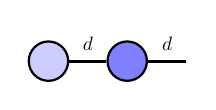
\begin{tikzpicture}[baseline=-0.1ex]
    \tikzset{tensor/.style = {minimum size = 0.5cm,shape = circle,thick,draw=black,inner sep = 0pt}, edge/.style = {thick,line width=.4mm},every loop/.style={}}
    \def\x{6}
    \def\y{0}
    \node[tensor,fill=blue!20!white] (x) at (\x+1,\y) {$\xb$};
    \node[tensor,fill=blue!50!white] (A) at (\x+2,\y) {$\Ab$};
    \draw[edge] (A) -- (x)node [midway, above] {\scalebox{0.7}{\dimcolor{$d$}}};
    \draw[edge] (A) -- (\x+2.75,\y)node [midway, above] {\scalebox{0.7}{\dimcolor{$d$}}};
    \end{tikzpicture}\\  
&=
    \Ab\xb + \Ab^\ts\xb = (\Ab\xb+\Ab^\ts)\xb.
\end{align*}
    \item 
设 $\Xb\in\RR^{n\times m},~\Wb\in\RR^{m\times n}$
    \begin{align*}
    \frac{\partial\norm{\Xb\Wb - \Yb}^2_F}{\partial \Wb}
&= 
    \frac{\partial\tr(\Wb^\ts\Xb^\ts\Xb\Wb)}{\partial\Wb}\\
&= 
    \frac{\partial\left( 
\begin{tikzpicture}[baseline=-0.1ex]
    \tikzset{tensor/.style = {minimum size = 0.5cm,shape = circle,thick,draw=black,inner sep = 0pt}, edge/.style = {thick,line width=.4mm},every loop/.style={}}
    \def\x{6}
    \def\y{0}
    \node[tensor,fill=red!20!white] (Wt) at (\x+1,\y) {$\Wb$};
    \node[tensor,fill=red!50!white] (Xt) at (\x+2,\y) {$\Xb$};
    \node[tensor,fill=red!50!white] (X) at (\x+3,\y) {$\Xb$};
    \node[tensor,fill=red!20!white] (W) at (\x+4,\y) {$\Wb$};
    \draw[edge] (Wt) -- (Xt)node [midway, above] {\scalebox{0.7}{\dimcolor{$m$}}};
    \draw[edge] (Xt) -- (X)node [midway, above] {\scalebox{0.7}{\dimcolor{$n$}}};
    \draw[edge] (X) -- (W)node [midway, above] {\scalebox{0.7}{\dimcolor{$n$}}};
    \draw[edge] (Wt) to [out=145,in=35, distance=1cm] (W);
    \end{tikzpicture}\right)}{\partial\left(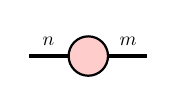
\begin{tikzpicture}[baseline=-0.1ex]
    \tikzset{tensor/.style = {minimum size = 0.5cm,shape = circle,thick,draw=black,inner sep = 0pt}, edge/.style = {thick,line width=.4mm},every loop/.style={}}
    \def\x{6}
    \def\y{0}   
    \node[tensor,fill=red!20!white] (W) at (\x+4,\y) {$\Wb$};
    \draw[edge] (W) -- (\x+4.75,\y)node [midway, above] {\scalebox{0.7}{\dimcolor{$m$}}};
    \draw[edge] (W) -- (\x+3.25,\y)node [midway, above] {\scalebox{0.7}{\dimcolor{$n$}}};
    \end{tikzpicture}\right)}\\
&=
    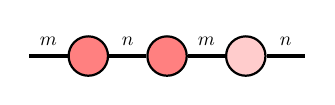
\begin{tikzpicture}[baseline=-0.1ex]
    \tikzset{tensor/.style = {minimum size = 0.5cm,shape = circle,thick,draw=black,inner sep = 0pt}, edge/.style = {thick,line width=.4mm},every loop/.style={}}
    \def\x{6}
    \def\y{0}
    \node[tensor,fill=red!50!white] (Xt) at (\x+2,\y) {$\Xb$};
    \node[tensor,fill=red!50!white] (X) at (\x+3,\y) {$\Xb$};
    \node[tensor,fill=red!20!white] (W) at (\x+4,\y) {$\Wb$};
    \draw[edge] (Xt) -- (\x+1.25,\y)node [midway, above] {\scalebox{0.7}{\dimcolor{$m$}}};
    \draw[edge] (Xt) -- (X)node [midway, above] {\scalebox{0.7}{\dimcolor{$n$}}};
    \draw[edge] (X) -- (W)node [midway, above] {\scalebox{0.7}{\dimcolor{$m$}}};
    \draw[edge] (W) -- (\x+4.75,\y)node [midway, above] {\scalebox{0.7}{\dimcolor{$n$}}};
    \end{tikzpicture}
+
    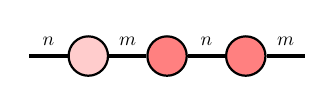
\begin{tikzpicture}[baseline=-0.1ex]
    \tikzset{tensor/.style = {minimum size = 0.5cm,shape = circle,thick,draw=black,inner sep = 0pt}, edge/.style = {thick,line width=.4mm},every loop/.style={}}
    \def\x{6}
    \def\y{0}
    \node[tensor,fill=red!20!white] (Wt) at (\x+1,\y) {$\Wb$};
    \node[tensor,fill=red!50!white] (Xt) at (\x+2,\y) {$\Xb$};
    \node[tensor,fill=red!50!white] (X) at (\x+3,\y) {$\Xb$};
    \draw[edge] (Wt) -- (Xt)node [midway, above] {\scalebox{0.7}{\dimcolor{$m$}}};
    \draw[edge] (Xt) -- (X)node [midway, above] {\scalebox{0.7}{\dimcolor{$n$}}};
    \draw[edge] (Wt) -- (\x+0.25,\y)node [midway, above] {\scalebox{0.7}{\dimcolor{$n$}}};
    \draw[edge] (X) -- (\x+3.75,\y)node [midway, above] {\scalebox{0.7}{\dimcolor{$m$}}};    
    \end{tikzpicture}\\
&=
2\Xb^\ts\Xb\Wb.
\end{align*}
\end{itemize}
本章最后给出张量网络梯度的若干应用。
\subsection{应用}
张量网络梯度的应用十分广泛，这里着重介绍两个典型例子。 

我们先简要介绍损失函数的概念，并说明链式法则如何方便地用于涉及张量与雅可比张量的表达式。损失函数 $L:S\times S\to \RR^{\geq 0}$ 用于度量计算模型、算法或决策过程在给出输出 $\hat{y}\in S$ 作为真值 $y\in S$ 的预测时所产生的误差或代价。许多学习与优化算法的目标就是最小化这一损失。一种做法是用 Frobenius 范数来度量预测输出与真值之差。当输入与输出都是张量时，可由雅可比张量算出所需梯度，从而最小化该 Frobenius 范数。设 $\At\in\RR^{d_1\times d_2\times d_3}$ 为真值，$\Tt\in\RR^{d_1\times d_2\times d_3}$ 为预测输出。利用定理~\ref{thm:gradients}，损失 $L = \norm{\At-\Tt}_F^2$ 的梯度可写为：
    \begin{align*}
        \frac{\partial\norm{\At-\Tt}_F^2}{\partial\Tt} 
        &=
        \frac{\partial}{\partial\Tt}\left(\norm{\At}_F^2 + \norm{\Tt}_F^2 - 2\langle\At,\Tt\rangle\right)\\
        &= 
    \frac{\partial}{\partial\Tt}\left(\begin{tikzpicture}[baseline=\baseline]
    \tikzset{tensor/.style = {minimum size = 0.5cm,shape = circle,thick,draw=black,inner sep = 0pt}, edge/.style = {thick,line width=.4mm},every loop/.style={}}
    \def\y{0}
    \def\x{0}
    \node[tensor,fill=green!50!red!50!white] (St) at (\x,\y){\scalebox{0.85}{$\Tt$}};
    \node[tensor,fill=green!50!red!50!white] (Tt) at (\x+1,\y){\scalebox{0.85}{$\Tt$}};
    \draw[edge] (St) -- (Tt);
    \draw[edge] (St) to [out=45,in=135] (Tt);
    \draw[edge] (St) to [out=-45,in=-135] (Tt);
    \node[draw=none] () at (\x+0.5,\y+0.5) {\scalebox{0.7}{\dimcolor{$d_1$}}};
    \node[draw=none] () at (\x+0.5,\y+0.15) {\scalebox{0.7}{\dimcolor{$d_2$}}};
    \node[draw=none] () at (\x+0.5,\y-0.5) {\scalebox{0.7}{\dimcolor{$d_3$}}};
\end{tikzpicture}
-2
~
\begin{tikzpicture}[baseline=\baseline]
    \tikzset{tensor/.style = {minimum size = 0.5cm,shape = circle,thick,draw=black,inner sep = 0pt}, edge/.style = {thick,line width=.4mm},every loop/.style={}}
    \def\y{0}
    \def\x{0}
    \node[tensor,fill=blue!40!red!20!white] (St) at (\x,\y){\scalebox{0.85}{$\At$}};
    \node[tensor,fill=green!50!red!50!white] (Tt) at (\x+1,\y){\scalebox{0.85}{$\Tt$}};
    \draw[edge] (St) -- (Tt);
    \draw[edge] (St) to [out=45,in=135] (Tt);
    \draw[edge] (St) to [out=-45,in=-135] (Tt);
    \node[draw=none] () at (\x+0.5,\y+0.5) {\scalebox{0.7}{\dimcolor{$d_1$}}};
    \node[draw=none] () at (\x+0.5,\y+0.15) {\scalebox{0.7}{\dimcolor{$d_2$}}};
    \node[draw=none] () at (\x+0.5,\y-0.5) {\scalebox{0.7}{\dimcolor{$d_3$}}};
\end{tikzpicture}
\right)\\
&=
\left(\begin{tikzpicture}[baseline=\baseline]
    \tikzset{tensor/.style = {minimum size = 0.5cm,shape = circle,thick,draw=black,inner sep = 0pt}, edge/.style = {thick,line width=.4mm},every loop/.style={}}
    \def\y{0}
    \def\x{0}
    \node[tensor,fill=green!50!red!50!white] (Tt) at (\x,\y){\scalebox{0.85}{$\Tt$}};
    \draw[edge](Tt) -- (\x+0.85,\y)node[midway, above]{\edgelabel{$d_2$}};
    \draw[edge](Tt) -- (\x-0.85,\y)node[midway, above]{\edgelabel{$d_1$}};
    \draw[edge](Tt) -- (\x,\y-0.85)node[midway, left]{\edgelabel{$d_3$}};
    \end{tikzpicture}
+
\begin{tikzpicture}[baseline=\baseline]
    \tikzset{tensor/.style = {minimum size = 0.5cm,shape = circle,thick,draw=black,inner sep = 0pt}, edge/.style = {thick,line width=.4mm},every loop/.style={}}
    \def\y{0}
    \def\x{0}
    \node[tensor,fill=green!50!red!50!white] (Tt) at (\x,\y){\scalebox{0.85}{$\Tt$}};
    \draw[edge](Tt) -- (\x+0.85,\y)node[midway, above]{\edgelabel{$d_2$}};
    \draw[edge](Tt) -- (\x-0.85,\y)node[midway, above]{\edgelabel{$d_1$}};
    \draw[edge](Tt) -- (\x,\y-0.85)node[midway, left]{\edgelabel{$d_3$}};
    \end{tikzpicture}
-2~~
\begin{tikzpicture}[baseline=\baseline]
    \tikzset{tensor/.style = {minimum size = 0.5cm,shape = circle,thick,draw=black,inner sep = 0pt}, edge/.style = {thick,line width=.4mm},every loop/.style={}}
    \def\y{0}
    \def\x{0}
    \node[tensor,fill=blue!40!red!20!white] (Tt) at (\x,\y){\scalebox{0.85}{$\At$}};
    \draw[edge](Tt) -- (\x+0.85,\y)node[midway, above]{\edgelabel{$d_2$}};
    \draw[edge](Tt) -- (\x-0.85,\y)node[midway, above]{\edgelabel{$d_1$}};
    \draw[edge](Tt) -- (\x,\y-0.85)node[midway, left]{\edgelabel{$d_3$}};
    \end{tikzpicture}\right)\\
&=
2\left(\begin{tikzpicture}[baseline=\baseline]
    \tikzset{tensor/.style = {minimum size = 0.5cm,shape = circle,thick,draw=black,inner sep = 0pt}, edge/.style = {thick,line width=.4mm},every loop/.style={}}
    \def\y{0}
    \def\x{0}
    \node[tensor,fill=green!50!red!50!white] (Tt) at (\x,\y){\scalebox{0.85}{$\Tt$}};
    \draw[edge](Tt) -- (\x+0.85,\y)node[midway, above]{\edgelabel{$d_2$}};
    \draw[edge](Tt) -- (\x-0.85,\y)node[midway, above]{\edgelabel{$d_1$}};
    \draw[edge](Tt) -- (\x,\y-0.85)node[midway, left]{\edgelabel{$d_3$}};
    \end{tikzpicture}
-
\begin{tikzpicture}[baseline=\baseline]
    \tikzset{tensor/.style = {minimum size = 0.5cm,shape = circle,thick,draw=black,inner sep = 0pt}, edge/.style = {thick,line width=.4mm},every loop/.style={}}
    \def\y{0}
    \def\x{0}
    \node[tensor,fill=blue!40!red!20!white] (Tt) at (\x,\y){\scalebox{0.85}{$\At$}};
    \draw[edge](Tt) -- (\x+0.85,\y)node[midway, above]{\edgelabel{$d_2$}};
    \draw[edge](Tt) -- (\x-0.85,\y)node[midway, above]{\edgelabel{$d_1$}};
    \draw[edge](Tt) -- (\x,\y-0.85)node[midway, left]{\edgelabel{$d_3$}};
    \end{tikzpicture}\right).
\end{align*}
链式法则很容易推广到涉及张量变量的表达式。例如，考虑任意损失函数 $\mathcal{ L}: \mathbb{R}^{d_1\times \cdots \times d_N} \to \mathbb{R}$，我们希望它在 $N$ 阶张量输入 $\Tt$ 上被最小化。再设该张量输入以张量网络的形式参数化，其中 $\Gt \in \mathbb{R}^{m_1\times \cdots \times m_M}$ 是一个 $M$ 阶核心张量。要计算 $\mathcal L$ 关于 $\Gt$ 的雅可比张量，可如下使用链式法则： 
$$\frac{\partial  \mathcal L}{\partial\Gt} 
=
\frac{\partial \mathcal L}{\partial \Tt }\frac{\partial\Tt}{\partial\Gt}  $$
其中 $\frac{\partial  \mathcal L}{\partial\Gt}$ 的尺寸为 $m_1\times\cdots \times m_M$，$\frac{\partial  \mathcal L}{\partial \Tt }$ 的尺寸为%
\footnote{严格来说，$\frac{\partial  \mathcal L}{\partial\Gt}$ 的形状为 $1\times m_1 \cdots \times m_M$，$\frac{\partial  \mathcal L}{\partial \Tt }$ 的形状为 $1\times d_1\times \cdots \times d_N$，只是维度为 $1$ 的第一个平凡模自然被省略了。}
$d_1\times \cdots \times d_N$，而 $\frac{\partial\Tt}{\partial\Gt} $ 的尺寸为 $d_1\times \cdots \times d_N \times m_1 \cdots \times m_M$。$\frac{\partial  \mathcal L}{\partial \Tt }$ 与 $\frac{\partial\Tt}{\partial\Gt}  $ 之间的乘积默认理解为：将 $\frac{\partial  \mathcal L}{\partial \Tt }$ 的 $M$ 个模与 $\frac{\partial\Tt}{\partial\Gt}  $ 的前 $M$ 个模相收缩。

有了这些工具，我们就可以用两个应用来结束本章，它们都涉及张量网络的梯度计算。 
\begin{itemize}
\item\textbf{用梯度下降求 CP 分解} 要求张量 $\Tt\in\RR^{d_1\times\cdots\times d_N}$ 的近似 CP 分解~(见第~\ref{sec:cp-decomposition}~节)，可用梯度下降最小化损失 $L = \norm{\Tt-\CP{\Gb_1,\cdots,\Gb_N}}^2_F$。这里 $\CP{\Gb_1,\cdots,\Gb_N}$ 表示 CP 分解，其中 $\Gb_1,\cdots,\Gb_N$ 为因子矩阵。为对因子矩阵作优化，可对损失函数施加梯度下降。例如在 $N=3$ 时，为求 $\Gb_1$，应用链式法则可写 $\frac{\partial L}{\partial\Gb_1} = \frac{\partial L}{\partial\CP{\Gb_1,\Gb_2,\Gb_3}}\frac{\partial\CP{\Gb_1,\Gb_2,\Gb_3}}{\partial\Gb_1}$，其中 $\frac{\partial L}{\partial\CP{\Gb_1,\Gb_2,\Gb_3}}= 2(\Tt-\CP{\Gb_1,\Gb_2,\Gb_3})\in\RR^{d_1\times d_2\times d_3}$，且 
\begin{align*}
\frac{\partial\CP{\Gb_1,\Gb_2,\Gb_3}}{\partial\Gb_1}
=
\begin{tikzpicture}[baseline=\baseline]
    \tikzset{tensor/.style = {minimum size = 0.5cm,shape = circle,thick,draw=black,inner sep = 0pt}, edge/.style   = {thick,line width=.4mm},every loop/.style={}}
    \def\y{0}
    \def\x{0}
 \node[tensor,fill=blue!50!white] (G2) at (\x+1,\y){$\Gb_2$};
   \node[tensor,fill=blue!20!white] (G3) at (\x+2,\y){$\Gb_3$};
    \draw  node[fill = black,circle,inner sep=0pt,minimum size=4pt] (m) at (\x+1,\y+1) {};
    \draw[edge] (m) -- (\x,\y+0.1) node [midway,left] {\edgelabel{$R$}};
    \draw[edge] (G2) -- (m)node [midway,left] {\edgelabel{$R$}};
    \draw[edge] (G3) -- (m)node [midway,right] {\edgelabel{$R$}};
    \draw[edge](\x,\y-0.1) -- (\x,\y-0.7) node [midway,right] {\edgelabel{$d_1$}};
    \draw[edge](G2) -- (\x+1,\y-0.7)node [midway,left] {\edgelabel{$d_2$}};
    \draw[edge](G3) -- (\x+2,\y-0.7) node [midway,left] {\edgelabel{$d_3$}};
\end{tikzpicture}\in\RR^{d_1\times d_2\times d_3\times R}.
\end{align*}
观察所得的张量网络可知，它能用矩阵化与 Khatri-Rao 积表示：
\begin{align*}
  \frac{\partial L}{\partial\Gb_1} 
&=
\frac{\partial L}{\partial\CP{\Gb_1,\Gb_2,\Gb_3}}\frac{\partial\CP{\Gb_1,\Gb_2,\Gb_3}}{\partial\Gb_1}\\
&=
\begin{tikzpicture}[baseline=-0.5ex]
    \tikzset{tensor1/.style = {minimum width = 3cm,minimum height = 0.6cm,shape = rounded rectangle,thick,draw=black,inner sep = 0pt}, edge/.style = {thick,line width=.4mm},every loop/.style={}}
     \tikzset{tensor2/.style = {minimum size = 0.5cm,shape = circle,thick,draw=black,inner sep = 0pt}, edge/.style   = {thick,line width=.4mm},every loop/.style={}}
    \def\y{1}
    \def\x{0}
    \node[tensor1,fill=blue!45!red!20!white] (Tt) at (\x,\y){$2(\Tt-\CP{\Gb_1,\Gb_2,\Gb_3})$};
    \node[tensor2,fill=blue!50!white] (G2) at (\x,\y-1){$\Gb_2$};
   \node[tensor2,fill=blue!20!white] (G3) at (\x+1,\y-1){$\Gb_3$};
    \draw  node[fill = black,circle,inner sep=0pt,minimum size=4pt] (m) at (\x+0.5,\y-1.85) {};
    \draw[edge](G2)--(m)node [midway,left] {\edgelabel{$R$}};
    \draw[edge](G3)--(m)node [midway,right] {\edgelabel{$R$}};    \draw[edge](Tt)--(G2)node [midway,left] {\edgelabel{$d_2$}};
    \draw[edge](\x+1,\y-0.3)--(G3)node [midway,left] {\edgelabel{$d_3$}};
    \draw[edge](m)--(\x+0.5,\y-2.25)node [midway,left] {\edgelabel{$R$}};
    \draw[edge](\x-0.75,\y-0.3) -- (\x-0.75,\y-2.25)node [midway,left] {\edgelabel{$d_1$}};
\end{tikzpicture}\\
&=\begin{tikzpicture}[baseline=-0.5ex]
    \tikzset{tensor/.style = {minimum width = 3cm,minimum height = 0.6cm,shape = rounded rectangle,thick,draw=black,inner sep = 0pt}, edge/.style = {thick,line width=.4mm},every loop/.style={}}
    \def\y{1}
    \def\x{0}
    \node[tensor,fill=blue!45!red!20!white] (Tt) at (\x,\y){$2(\Tt-\CP{\Gb_1,\Gb_2,\Gb_3})$};
    \node[tensor,fill=blue!25!red!45!white] (Gt) at (\x+1,\y-1){$\Gb_2\krao\Gb_3$};
    \draw[edge](\x+0.5,\y-0.3) -- (\x+0.5,\y-0.7);
    \draw[edge](\x+0.6,\y-0.3) -- (\x+0.6,\y-0.7)node [midway,right] {\edgelabel{$d_2d_3$}};
    \draw[edge](\x-0.75,\y-0.3) -- (\x-0.75,\y-2)node [midway,left] {\edgelabel{$d_1$}};
    \draw[edge](\x+0.85,\y-1.3) -- (\x+0.85,\y-2)node [midway,left] {\edgelabel{$R$}};
\end{tikzpicture}\\
&=
2(\Tt-\CP{\Gb_1,\Gb_2,\Gb_3})_{(1)}(\Gb_2\krao\Gb_3)
\in\RR^{d_1\times R}.
\end{align*}
 \item\textbf{机器学习} 为压缩神经网络，可用张量分解来参数化全连接层的稠密权重矩阵，从而减少内存占用~\citep{novikov2015tensorizing}。设 $\Wb\in\RR^{P\times D}$ 为权重矩阵，$\xb\in\RR^{D}$ 为神经网络某一层的输入向量。输出 $\yb\in\RR^{P}$ 由权重矩阵 $\Wb$ 与输入向量 $\xb$ 收缩而得。 
    设 $P = \Pi_{i=1}^N{p_i}$ 且 $D =\Pi_{i=1}^Nd_i$。将 $\Wb$ 与 $\xb$ 重排为张量后，便有
\begin{align*}
    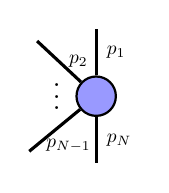
\begin{tikzpicture}[baseline=-0.1ex]
    \tikzset{tensor/.style = {minimum size = 0.5cm,shape = circle,thick,draw=black,inner sep = 0pt}, edge/.style = {thick,line width=.4mm},every loop/.style={}}
    \def\x{6}
    \def\y{0}
    \node[tensor,fill=blue!40!white] (y) at (\x,\y) {$\Yt$};
    \draw[edge](y)--(\x,\y+0.85)node [midway,right] {\scalebox{0.7}{\dimcolor{$p_1$}}};
    \draw[edge](y)--(\x-0.75,\y+0.7)node [midway,right=-0.01cm] {\scalebox{0.7}{\dimcolor{$p_2$}}};
    \draw[edge](y)--(\x-0.85,\y-0.7)node [very near end,right] {\scalebox{0.7}{\dimcolor{$p_{N-1}$}}};
    \draw[edge](y)--(\x,\y-0.85)node [midway,right] {\scalebox{0.7}{\dimcolor{$p_N$}}};
    \node[draw=none] at (\x-0.5,\y+0.1){$\vdots$};
    \end{tikzpicture}
=\sum_{d_1,\cdots,d_N}\Wt_{p_1,\cdots, p_N,d_1,\cdots, d_N}\Xt_{d_1,\cdots, d_N} =
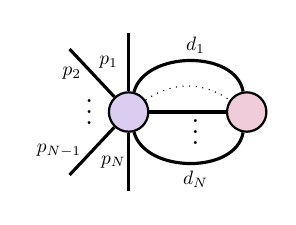
\begin{tikzpicture}[baseline=-0.1ex]
    \tikzset{tensor/.style = {minimum size = 0.5cm,shape = circle,thick,draw=black,inner sep = 0pt}, edge/.style = {thick,line width=.4mm},every loop/.style={}}
    \def\x{6}
    \def\y{0}
    \node[tensor,fill=red!30!blue!20!white] (w) at (\x,\y) {$\Wt$};
    \node[tensor,fill=blue!30!red!20!white] (x) at (\x+1.5,\y) {$\Xt$};
    \draw[edge](w)--(x);
    \draw[edge](w)--(\x,\y+1)node [midway,left] {\scalebox{0.7}{\dimcolor{$p_1$}}};
    \draw[edge](w)--(\x-0.75,\y+0.8)node [midway,left] {\scalebox{0.7}{\dimcolor{$p_2$}}};
    \draw[edge](w)--(\x-0.75,\y-0.8)node [midway,left] {\scalebox{0.7}{\dimcolor{$p_{N-1}$}}};
    \draw[edge](w)--(\x,\y-1)node [midway,left=-0.1cm] {\scalebox{0.7}{\dimcolor{$p_N$}}};
    \node[draw=none] at (\x-0.5,\y+0.1){$\vdots$};
   \draw[edge] (w) to [out=-75,in=-100] (x);
    \draw[edge] (w) to [out=75,in=100] (x);
    \draw[dotted] (w) to [out=35,in=145] (x);
    \node[draw=none] at (\x+0.85,\y-0.15){$\vdots$};
    \node[draw=none] () at (\x+0.85,\y+0.85) {\scalebox{0.7}{\dimcolor{$d_1$}}};
    (\x+1.2,\y-0.2){$\vdots$};
    \node[draw=none] () at (\x+0.85,\y-0.85) {\scalebox{0.7}{\dimcolor{$d_N$}}};
\end{tikzpicture}.
\end{align*}
为简单起见，下面只考虑 $N=4$ 的情形。文献~\citep{novikov2015tensorizing} 的作者提出以 MPO 格式参数化 $\Wt$~(见第~\ref{sec:efficient-operations}~节)，即 
$\Wt = 
\begin{tikzpicture}[baseline=\baseline]
    \tikzset{tensor/.style = {minimum size = 0.5cm,shape = circle,thick,draw=black,inner sep = 0pt}, edge/.style   = {thick,line width=.4mm},every loop/.style={}}
    \def\y{0}
    \def\x{0}
  \node[tensor,fill=red!30!white] (G1) at (\x,\y){$\Gt_1$};
  \node[tensor,fill=red!50!white] (G2) at (\x+1,\y){\scalebox{0.85}{$\Gt_2$}};
  \node[tensor,fill=blue!30!white] (G3) at (\x+2,\y){$\Gt_3$};
  \node[tensor,fill=blue!50!white] (G4) at (\x+3,\y){$\Gt_4$};
    \draw[edge](G1) -- (\x,\y-0.85)node [midway,left] {\edgelabel{$d_1$}};
    \draw[edge](G2) -- (\x+1,\y-0.85)node [midway,left] {\edgelabel{$d_2$}};
     \draw[edge](G3) -- (\x+2,\y-0.85)node [midway,left] {\edgelabel{$d_3$}};
    \draw[edge](G4) -- (\x+3,\y-0.85)node [midway,left] {\edgelabel{$d_4$}};
    \draw[edge](G1) -- (G2) node [midway,above] {\edgelabel{$R_1$}};
    \draw[edge](G2) -- (G3) node [midway,above] {\edgelabel{$R_2$}};
    \draw[edge](G3) -- (G4) node [midway,above] {\edgelabel{$R_3$}};
    \draw[edge](G1) -- (\x,\y+0.85)node [midway,left] {\edgelabel{$p_1$}};
    \draw[edge](G2) -- (\x+1,\y+0.85)node [midway,left] {\edgelabel{$p_2$}};
    \draw[edge](G3) -- (\x+2,\y+0.85)node [midway,left] {\edgelabel{$p_3$}};
    \draw[edge](G4) -- (\x+3,\y+0.85)node [midway,left] {\edgelabel{$p_4$}};
\end{tikzpicture}.$
在反向传播步骤中，由于要更新的是权重矩阵，就需要对全部核心张量作优化。按链式法则，对 $i\in[4]$ 有 $\frac{\partial L}{\partial \Gt_i} = \frac{\partial L}{\partial \Yt}\frac{\partial\Yt}{\partial\Gt_i}$，其中 $L$ 表示损失函数。例如 $i=2$ 时，需求 $\Yt$ 关于 $\Gt_2$ 的导数。利用定理~\ref{thm:gradients}，只需从张量网络中删去 $\Gt_2$ 便可得到结果：
\begin{align*}
\frac{\partial\Yt}{\partial\Gt_2} 
&=
\frac{\partial\left(\begin{tikzpicture}[baseline=\baseline]
    \tikzset{tensor/.style = {minimum size = 0.5cm,shape = circle,thick,draw=black,inner sep = 0pt}, edge/.style   = {thick,line width=.4mm},every loop/.style={}}
    \def\y{0}
    \def\x{0}
  \node[tensor,fill=red!30!white] (G1) at (\x,\y){$\Gt_1$};
  \node[tensor,fill=red!50!white] (G2) at (\x+1,\y){\scalebox{0.85}{$\Gt_2$}};
  \node[tensor,fill=blue!30!white] (G3) at (\x+2,\y){$\Gt_3$};
  \node[tensor,fill=blue!50!white] (G4) at (\x+3,\y){$\Gt_4$};
  \node[tensor,fill=blue!30!red!20!white] (x) at (\x+1.5,\y-1.5) {$\Xt$};
    \draw[edge](G1) -- (\x,\y-0.85)node [midway,left] {\edgelabel{$d_1$}};
    \draw[edge](x)--(\x,\y-0.85);
    \draw[edge](G2) -- (\x+1,\y-0.85)node [midway,left] {\edgelabel{$d_2$}};
    \draw[edge](x)--(\x+1,\y-0.85);
     \draw[edge](G3) -- (\x+2,\y-0.85)node [midway,left] {\edgelabel{$d_3$}};
    \draw[edge](x)--(\x+2,\y-0.85);
    \draw[edge](G4) -- (\x+3,\y-0.85)node [midway,left] {\edgelabel{$d_4$}};
    \draw[edge](x)--(\x+3,\y-0.85);
    \draw[edge](G1) -- (G2) node [midway,above] {\edgelabel{$R_1$}};
    \draw[edge](G2) -- (G3) node [midway,above] {\edgelabel{$R_2$}};
    \draw[edge](G3) -- (G4) node [midway,above] {\edgelabel{$R_3$}};
    \draw[edge](G1) -- (\x,\y+0.85)node [midway,left] {\edgelabel{$p_1$}};
    \draw[edge](G2) -- (\x+1,\y+0.85)node [midway,left] {\edgelabel{$p_2$}};
    \draw[edge](G3) -- (\x+2,\y+0.85)node [midway,left] {\edgelabel{$p_3$}};
    \draw[edge](G4) -- (\x+3,\y+0.85)node [midway,left] {\edgelabel{$p_4$}};
\end{tikzpicture}\right)}{\partial\Gt_2}\\
&=
\begin{tikzpicture}[baseline=\baseline]
    \tikzset{tensor/.style = {minimum size = 0.5cm,shape = circle,thick,draw=black,inner sep = 0pt}, edge/.style   = {thick,line width=.4mm},every loop/.style={}}
    \def\y{-1}
    \def\x{0}
  \node[tensor,fill=red!30!white] (G1) at (\x,\y+1.5){$\Gt_1$};
    \node[tensor,fill=blue!30!white] (G3) at (\x+2,\y+1.5){$\Gt_3$};
  \node[tensor,fill=blue!50!white] (G4) at (\x+3,\y+1.5){$\Gt_4$};
  \node[tensor,fill=blue!30!red!20!white] (x) at (\x+1.5,\y) {$\Xt$};
    \draw[edge](G1) -- (\x,\y+0.85)node [midway,left] {\edgelabel{$d_1$}};
    \draw[edge](x)--(\x,\y+0.85);
    \draw[edge](\x+1,\y+1.35) -- (\x+1,\y+0.85)node [midway,left] {\edgelabel{$d_2$}};
    \draw[edge](x)--(\x+1,\y+0.85);
     \draw[edge](G3) -- (\x+2,\y+0.85)node [midway,left] {\edgelabel{$d_3$}};
    \draw[edge](x)--(\x+2,\y+0.85);
    \draw[edge](G4) -- (\x+3,\y+0.85)node [midway,left] {\edgelabel{$d_4$}};
    \draw[edge](x)--(\x+3,\y+0.85);
    \draw[edge](G3) -- (G4) node [midway,above] {\edgelabel{$R_3$}};
    \draw[edge](G1) -- (\x,\y+2.35)node [midway,left] {\edgelabel{$p_1$}};
    \draw[edge](G3) -- (\x+2,\y+2.35)node [midway,left] {\edgelabel{$p_3$}};
    \draw[edge](G4) -- (\x+3,\y+2.35)node [midway,left] {\edgelabel{$p_4$}};
    \draw[edge](G1)--(\x+0.85,\y+1.5) node [midway,above] {\edgelabel{$R_1$}};
    \draw[edge](G3)--(\x+1.25,\y+1.5) node [midway,above] {\edgelabel{$R_2$}};
    \draw[edge](\x+1,\y+1.6)--(\x+1,\y+2.35) node [midway,left] {\edgelabel{$p_2$}};
\end{tikzpicture}\in\RR^{p_1\times R_1\times p_2\times R_2\times p_3\times p_4\times d_2}.
\end{align*}
于是损失的梯度为
\begin{align*}
    \frac{\partial L}{\partial\Gt_2} = \frac{\partial L}{\partial\Yt}\frac{\partial \Yt}{\partial\Gt_2}
    =
    \begin{tikzpicture}[baseline=\baseline]
    \tikzset{tensor/.style = {minimum size = 0.5cm,shape = circle,thick,draw=black,inner sep = 0pt}, edge/.style   = {thick,line width=.4mm},every loop/.style={}}
    \def\y{-1.5}
    \def\x{0}
    \node[tensor,fill=green!30!white] (L) at (\x+1.5,\y+3.25){$\frac{\partial L}{\partial\Yt}$};
  \node[tensor,fill=red!30!white] (G1) at (\x,\y+1.5){$\Gt_1$};
    \node[tensor,fill=blue!30!white] (G3) at (\x+2,\y+1.5){$\Gt_3$};
  \node[tensor,fill=blue!50!white] (G4) at (\x+3,\y+1.5){$\Gt_4$};
  \node[tensor,fill=blue!30!red!20!white] (x) at (\x+1.5,\y) {$\Xt$};
    \draw[edge](G1) -- (\x,\y+0.85)node [midway,left] {\edgelabel{$d_1$}};
    \draw[edge](x)--(\x,\y+0.85);
    \draw[edge](\x+1,\y+1.35) -- (\x+1,\y+0.85)node [midway,left] {\edgelabel{$d_2$}};
    \draw[edge](x)--(\x+1,\y+0.85);
     \draw[edge](G3) -- (\x+2,\y+0.85)node [midway,left] {\edgelabel{$d_3$}};
    \draw[edge](x)--(\x+2,\y+0.85);
    \draw[edge](G4) -- (\x+3,\y+0.85)node [midway,left] {\edgelabel{$d_4$}};
    \draw[edge](x)--(\x+3,\y+0.85);
    \draw[edge](G3) -- (G4) node [midway,above] {\edgelabel{$R_3$}};
    \draw[edge](G1) -- (\x,\y+2.35)node [midway,left] {\edgelabel{$p_1$}};
    \draw[edge](L)--(\x,\y+2.35);
    \draw[edge](G3) -- (\x+2,\y+2.35)node [midway,left] {\edgelabel{$p_3$}};
    \draw[edge](L)--(\x+2,\y+2.35);
    \draw[edge](G4) -- (\x+3,\y+2.35)node [midway,left] {\edgelabel{$p_4$}};
    \draw[edge](L)--(\x+3,\y+2.35);
    \draw[edge](G1)--(\x+0.85,\y+1.5) node [midway,above] {\edgelabel{$R_1$}};
    \draw[edge](G3)--(\x+1.25,\y+1.5) node [midway,above] {\edgelabel{$R_2$}};
    \draw[edge](\x+1,\y+1.6)--(\x+1,\y+2.35) 
    node [midway,left] {\edgelabel{$p_2$}};
    \draw[edge](L)--(\x+1,\y+2.35);
\end{tikzpicture}\in\RR^{R_1\times p_2\times R_2\times d_2}.
\end{align*}

\end{itemize}






